\documentclass{article}

%%%%%%%%%%%%%%%%%%%%%%%%%%%%%%%%%%%%%%%%%%%%%%%%%%%%%%%%%%%%%%%%%%%%%%%%%%%
%%%%%%%%%%%%%%%%%%%%%%% Page Layout and Typography %%%%%%%%%%%%%%%%%%%%%%%
%%%%%%%%%%%%%%%%%%%%%%%%%%%%%%%%%%%%%%%%%%%%%%%%%%%%%%%%%%%%%%%%%%%%%%%%%%%

\usepackage[utf8]{inputenc}
\usepackage{geometry}
\usepackage{rotating}
\usepackage{indentfirst}
\usepackage{parskip}
\usepackage{pslatex}
\usepackage{setspace}
\geometry{
    left=1in,
    right=1in,
    top=0.8in,
    bottom=0.8in,
}


%%%%%%%%%%%%%%%%%%%%%%%%%%%%%%%%%%%%%%%%%%%%%%%%%%%%%%%%%%%%%%%%%%%%%%%%%%%
%%%%%%%%%%%%%%%%%%%%%%%% Figures, Captions, and Lists %%%%%%%%%%%%%%%%%%%%%
%%%%%%%%%%%%%%%%%%%%%%%%%%%%%%%%%%%%%%%%%%%%%%%%%%%%%%%%%%%%%%%%%%%%%%%%%%%

\usepackage{graphicx}
\usepackage{float}
\usepackage{array}
\usepackage{booktabs}
\usepackage[font=small, labelfont=bf]{caption}
\usepackage{subcaption}
\usepackage{enumitem} % set configuration for list


%%%%%%%%%%%%%%%%%%%%%%%%%%%%%%%%%%%%%%%%%%%%%%%%%%%%%%%%%%%%%%%%%%%%%%%%%%%
%%%%%%%%%%%%%%%%%%%%%%%%%%%% Math Packages %%%%%%%%%%%%%%%%%%%%%%%%%%%%%%%%
%%%%%%%%%%%%%%%%%%%%%%%%%%%%%%%%%%%%%%%%%%%%%%%%%%%%%%%%%%%%%%%%%%%%%%%%%%%

\usepackage{amsmath,amsthm,amssymb}
\usepackage{mathtools}
\usepackage{bm}
\usepackage{dsfont}


%%%%%%%%%%%%%%%%%%%%%%%%%%%%%%%%%%%%%%%%%%%%%%%%%%%%%%%%%%%%%%%%%%%%%%%%%%%
%%%%%%%%%%%%%%%%%%%%%%%%%%%% Title Helpers %%%%%%%%%%%%%%%%%%%%%%%%%%%%%%%%
%%%%%%%%%%%%%%%%%%%%%%%%%%%%%%%%%%%%%%%%%%%%%%%%%%%%%%%%%%%%%%%%%%%%%%%%%%%

\usepackage{titling}
\newcommand{\subtitle}[1]{
  \posttitle{
    \par\end{center}
    \begin{center}\large#1\end{center}\vspace{-3.5em}
    \vskip0.5em}
}


%%%%%%%%%%%%%%%%%%%%%%%%%%%%%%%%%%%%%%%%%%%%%%%%%%%%%%%%%%%%%%%%%%%%%%%%%%%
%%%%%%%%%%%%%%%%%%%%%%%%%%%%%%%% Colors %%%%%%%%%%%%%%%%%%%%%%%%%%%%%%%%%%%
%%%%%%%%%%%%%%%%%%%%%%%%%%%%%%%%%%%%%%%%%%%%%%%%%%%%%%%%%%%%%%%%%%%%%%%%%%%

\usepackage{xcolor}
\newcommand{\red}{\textcolor{red}}
\newcommand{\blue}{\textcolor{blue}}
\newcommand{\green}{\textcolor{green}}


%%%%%%%%%%%%%%%%%%%%%%%%%%%%%%%%%%%%%%%%%%%%%%%%%%%%%%%%%%%%%%%%%%%%%%%%%%%
%%%%%%%%%%%%%%%%%%%%%%%%%%%% Framed Blocks %%%%%%%%%%%%%%%%%%%%%%%%%%%%%%%%
%%%%%%%%%%%%%%%%%%%%%%%%%%%%%%%%%%%%%%%%%%%%%%%%%%%%%%%%%%%%%%%%%%%%%%%%%%%

% colored block, credit to Kevin Z. Lin
\definecolor{col0}{rgb}{0.950,0.930,0.855} %gray/beige
\usepackage{mdframed}
\newenvironment{block}
{	\begin{center}
    \vspace{1em}
   	\begin{mdframed}[
    backgroundcolor=col0,
    topline=false,
    bottomline=false,
    rightline=false,
    leftline=false,
    skipabove=20pt,  % space before
    skipbelow=20pt   % space after
    ]
}
{
   	\end{mdframed} 
   	\end{center}
}

% boxed text
\newenvironment{mybox}{%
  \par\addvspace{10pt}% space that survives right after \section
  \begin{mdframed}[skipabove=0pt,skipbelow=10pt]%
}{%
  \end{mdframed}%
}


%%%%%%%%%%%%%%%%%%%%%%%%%%%%%%%%%%%%%%%%%%%%%%%%%%%%%%%%%%%%%%%%%%%%%%%%%%%
%%%%%%%%%%%%%%%%%%%%%%%%% Theorem Environments %%%%%%%%%%%%%%%%%%%%%%%%%%%
%%%%%%%%%%%%%%%%%%%%%%%%%%%%%%%%%%%%%%%%%%%%%%%%%%%%%%%%%%%%%%%%%%%%%%%%%%%

% Define a custom theorem style that places the title on a separate line
\newtheoremstyle{break}
  {\topsep}   % Space above
  {\topsep}   % Space below
  {\itshape}  % Body font
  {}          % Indent amount
  {\bfseries} % Theorem head font
  {.}         % Punctuation after theorem head
  {\newline}  % Space after theorem head (THIS IS THE LINEBREAK)
  {}          % Theorem head spec

% Apply this style and define 'Fact'
\theoremstyle{break}
\newtheorem*{fact}{Fact} % Define an unnumbered 'Fact' environment
\newtheorem{Fact}{Fact}  % numbered environ


%%%%%%%%%%%%%%%%%%%%%%%%%%%%%%%%%%%%%%%%%%%%%%%%%%%%%%%%%%%%%%%%%%%%%%%%%%%
%%%%%%%%%%%%%%%%%%%%%%%%%%%%%%%%% Links %%%%%%%%%%%%%%%%%%%%%%%%%%%%%%%%%%%
%%%%%%%%%%%%%%%%%%%%%%%%%%%%%%%%%%%%%%%%%%%%%%%%%%%%%%%%%%%%%%%%%%%%%%%%%%%

\usepackage[colorlinks=true,
            linkcolor=blue,
            urlcolor=blue,
            citecolor=blue]{hyperref}


%%%%%%%%%%%%%%%%%%%%%%%%%%%%%%%%%%%%%%%%%%%%%%%%%%%%%%%%%%%%%%%%%%%%%%%%%%%
%%%%%%%%%%%%%%%%%%%%%%%%%%%%%%%% Notation %%%%%%%%%%%%%%%%%%%%%%%%%%%%%%%%%
%%%%%%%%%%%%%%%%%%%%%%%%%%%%%%%%%%%%%%%%%%%%%%%%%%%%%%%%%%%%%%%%%%%%%%%%%%%
% Number systems and common spaces
\newcommand{\R}{\ensuremath{\mathbb{R}}}
\newcommand{\Z}{\ensuremath{\mathbb{Z}}}
\newcommand{\N}{\ensuremath{\mathbb{N}}}
\newcommand{\E}{\ensuremath{\mathbb{E}}}
\newcommand{\F}{\ensuremath{\mathcal{F}}}

% Bold random vectors / matrices
\newcommand{\bX}{\ensuremath{\mathbf{X}}}
\newcommand{\bY}{\ensuremath{\mathbf{Y}}}
\newcommand{\bZ}{\ensuremath{\mathbf{Z}}}

% Basic math shortcuts
\newcommand{\st}{\ensuremath{\text{ s.t. }}}
\newcommand{\dd}{\ensuremath{\mathrm{d}}}

% Delimiters
\newcommand{\p}[1]{\ensuremath{\left(#1\right)}}
\newcommand{\br}[1]{\ensuremath{\left\{#1\right\}}}
\newcommand{\sbr}[1]{\ensuremath{\left[#1\right]}}
\newcommand{\abs}[1]{\ensuremath{\left|#1\right|}}
\newcommand{\norm}[1]{\ensuremath{\left\lVert#1\right\rVert}}
\newcommand{\ip}[1]{\ensuremath{\left\langle #1 \right\rangle}}
\newcommand{\ceil}[1]{\ensuremath{\left\lceil#1\right\rceil}}
\newcommand{\floor}[1]{\ensuremath{\left\lfloor#1\right\rfloor}}

% Probability and statistics
\newcommand{\Prob}[2]{\ensuremath{\mathbb{P}_{#1}\left(#2\right)}}
\newcommand{\Ind}[2]{\ensuremath{\mathbbm{1}_{#1}\left(#2\right)}}
\newcommand{\iid}{\ensuremath{\mathrm{i.i.d.}}}
\newcommand{\iidsim}{\ensuremath{\overset{\mathrm{i.i.d.}}{\sim}}}
\newcommand{\cdf}{\ensuremath{\mathrm{c.d.f.}}}
\newcommand{\pdf}{\ensuremath{\mathrm{p.d.f.}}}
\newcommand{\pmf}{\ensuremath{\mathrm{p.m.f.}}}
\DeclareMathOperator{\Var}{Var}
\DeclareMathOperator{\Cov}{Cov}
\DeclareMathOperator{\Bernoulli}{Bernoulli}
\DeclareMathOperator{\Binomial}{Binomial}
\DeclareMathOperator{\Geometric}{Geometric}
\DeclareMathOperator{\Multinomial}{Multinomial}
\DeclareMathOperator{\NegativeBinomial}{NegativeBinomial}

% Linear algebra and geometry
\DeclareMathOperator{\tr}{tr}
\DeclareMathOperator{\Span}{Span}
\DeclareMathOperator{\diag}{diag}
\DeclareMathOperator{\rank}{rank}
\DeclareMathOperator{\conv}{conv}
\DeclareMathOperator{\aff}{aff}
\newcommand{\op}{\ensuremath{\mathrm{op}}}

% Optimization
\DeclareMathOperator*{\argmax}{arg\,max}
\DeclareMathOperator*{\argmin}{arg\,min}


\author{Wenbin Wu}
\title{BIOS762 Review}


\begin{document}
\maketitle

% --- disclaimer ---
% Paragraph 1: role of these notes
The following notes are based on the lecture slides of BIOS761 (Advanced Probability and Statistical Inference II) at UNC Chapel Hill. They are compiled from the author's \emph{personal understanding} of the course material and aim to summarize the key results, highlight connections among the main concepts and theorems, and collect useful problem-solving strategies.

% Paragraph 2: suggested use
These notes are \emph{not} intended to be a comprehensive summary of the lecture slides, but rather a supplementary resource. They are most useful as a review document after a first pass through the lecture slides or as a quick reference while working through exam problems.

For simplicity, some notation differs from that used in the lecture slides. If any statement is unclear or appears incorrect, please verify it against the course materials and consult other reliable references. We also encourage the use of AI assistants together with these notes and the relevant course materials to clarify concepts, fill in omitted details, and answer questions that arise while studying.

% Paragraph 3: acknowledgment and contributions
We warmly welcome corrections, suggestions, and contributions from readers. 
If you would like to contribute, please submit a pull request through the GitHub repository: \url{https://github.com/WenbinWu2001/oh-my-qualify-theory}.

\tableofcontents
\newpage

% --- main content ---
\section{Decision Theory}
Statistical decision theory studies how to utilize sample information to make decisions such that risk is minimized. 
Its basic components are the statistical model $\{P_\theta:\theta\in\Theta\}$, the action space $\mathcal{A}$, and the loss function $L$. Bayesian decision theory additionally introduces a prior distribution $\Lambda$ on the parameter space $\Theta$.

\subsection{Decision problem}
\subsubsection{Basic elements}
\begin{itemize}
    \item unknown parameter (also called ``state of nature'') $\theta$. Denote parameter space as $\Theta$.
    \item samples $x$ of a random variable $X$ with distribution $P_\theta$. Denote sample space as $\mathcal{X}$.
    \item action (decision) $a$ with action space $\mathcal{A}$. In estimation problems, $\mathcal{A} = \Theta$.
    \item loss function $L:\Theta \times \mathcal{A} \to \R^+$ where $L(\theta, a)$ characterizes the consequence of decision $a$ when the parameter takes value $\theta$.
    \item decision rule/function: $d:\mathcal{X} \to \mathcal{A}$ where $d(x)$ is the action taken when $X=x$ is observed. Denote the set of all decision rules as $\mathcal{D}$. In estimation problems, a decision rule is called an estimator.
    \begin{itemize}
        \item non-randomized (deterministic): $d(x)$ takes a single value in $\mathcal{A}$.
        \item randomized: $d(x)$ is a probability distribution over the action space $\mathcal{A}$. $d(a|x): \mathcal{A} \times \mathcal{X} \to [0,1]$ is the probability of taking action $a$ when $X=x$ is observed. In this case, the loss function is $L(\theta, d(\cdot|x)) = \E_{a \sim p(a|x)}[L(\theta, a)]$ (i.e., expectation over the action space). Note that a non-randomized rule is just a randomized rule that assigns probability $1$ to a single action.
        \item If the action space $\mathcal{A}$ is convex and the loss function $L(\theta,a)$ is convex in the action $a$, then every randomized decision rule can be replaced by a nonrandomized rule that is at least as good -- and uniformly better when the loss is strictly convex. Under these conditions, it suffices to consider nonrandomized rules. (Caveat: These convexity conditions often fail when the action space is discrete or the loss is nonconvex, as commonly occurs in hypothesis-testing problems with $0$-$1$ loss.)
    \end{itemize}
    \item Any decision problem is defined by $(\Theta, \mathcal{A}, L)$, that is, states, actions, and a loss function.
\end{itemize}

\subsection{What are ``good'' decision rules?}
\subsubsection{Basic elements}
\begin{itemize}
    \item risk function $R:\Theta \times \mathcal{D} \to \R^+$ where $R(\theta,d) = \E_{X \sim P_\theta}[L(\theta, d(X)]$ is the expected loss of decision rule $d$ at parameter value $\theta$. \footnote{For randomized decision rules, $R(\theta,d) = \int_\mathcal{X}\int_\mathcal{A} L(\theta,a)p(a|x)p(x|\theta) dadx$ is a double integral over the sample space and action space. You can exchange the integrals to facilitate calculations.}
    \item A decision rule $d$ is \emph{inadmissible} if there exists a rule $d'$ such that $R(\theta, d') \leq R(\theta, d)$ for all $\theta$ and $R(\theta, d') < R(\theta, d)$ for some $\theta$. In other words, $d'$ is uniformly better than\footnote{More precisely, $d'$ is uniformly no worse than $d$ and strictly better for at least one $\theta$.}, or \emph{dominates}, $d$.
    \item A decision rule $d$ is \emph{admissible} if it is not inadmissible (i.e., there is no rule that dominates $d$). For a particular problem, there is usually a class of admissible decision rules which are best at different values of $\theta$.
    \item The class of admissible decision rules is often too large for practical optimization, so we restrict attention to a class $\mathcal{D}$ and seek an optimal rule within it. A decision rule $d$ is \emph{optimal} in $\mathcal{D}$ if $R(\theta, d) \leq R(\theta, d')$ for all $\theta \in \Theta$ and for all $d' \in \mathcal{D}$. In other words, $d$ achieves minimal risk everywhere in the parameter space $\Theta$.
\end{itemize}

In most problems, there is no optimal decision rule. Hence we use different principles to characterize optimality.

\subsubsection{Minimax principle} % move under Bayesian?
Minimax principle considers the worst-case risk in the parameter space $\Theta$. One decision rule $d_1$ is better than another $d_2$ if $\sup_{\theta\in \Theta} R(\theta,d_1) < \sup_{\theta\in \Theta} R(\theta,d_2)$.

A decision rule $d_M$ is \emph{minimax} if
\[
\sup_{\theta \in \Theta} R(\theta, d_M) = \inf_{d \in \mathcal{D}} \{\sup_{\theta \in \Theta} R(\theta, d)\}.
\]
In other words, among all decision rules in $\mathcal{D}$, $d_M$ has the smallest worst-case risk. The quantity on the right hand side is called the \emph{minimax value} of the problem.

\begin{mybox}
    \textbf{Fact 1:} If the minimax estimator is unique (i.e., uniquely achieves the minimax value), then it is admissible.
    
    \textbf{Fact 2:} Any estimator better than a minimax estimator is also minimax.
    \footnote{Here, ``better'' means pointwise no worse on $\Theta$. The two estimators have the same maximum risk, equal to the minimax value. If the maximum risk of the better estimator is \emph{attained}, their risks coincide at some parameter value at which the minimax value is attained.}
\end{mybox}

\subsubsection{Bayesian principle}
Bayesian principle considers the expected risk over a prior distribution on the parameter space $\Theta$, rather than seeing $\theta$ as an unknown but fixed parameter.


Denote $\Lambda$ as the prior distribution of $\theta$ over $\Theta$. The \emph{Bayes risk of $d$ with respect to a given prior $\Lambda$} is 
\[
R(\Lambda, d) = \E_{\theta \sim \Lambda}[R(\theta, d)].
\]

A \emph{Bayesian decision rule} with respect to $\Lambda$, denoted by $d_\Lambda$, is a rule achieving the minimal Bayes risk in $\mathcal{D}$, namely,
\[R(\Lambda, d_\Lambda) = \inf_{d\in \mathcal{D}} R(\Lambda, d).\]
The quantity on the right hand side is called the \emph{Bayes risk}. In estimation problems, we refer to the Bayes rule as the \emph{Bayes estimator} of $\theta$.

\textbf{Caveat:} Admissibility and minimaxity are frequentist concepts, defined independently of any prior distribution. In particular, neither the admissibility of a decision rule $d$ nor its minimax value depends on $\Lambda$. On the other hand, whether a rule is Bayes generally depends on the chosen prior.

\subsubsection{How to find a Bayes rule?}
Remember that the goal is to find the action $d(x)$ for each given $x\in \mathcal{X}$. Notice that the Bayes risk can be rewritten as
\[
R(\Lambda, d) 
= \int_\Theta 
\Big[ \int_\mathcal{X} L(\theta, d(x)) p(x|\theta) dx \Big]
\lambda(\theta) d\theta
= \int_\mathcal{X} 
\underbrace{\Big[\int_\Theta L(\theta, d(x)) p(\theta|x) d\theta \Big]}_{\text{posterior expected loss}}
p(x) dx,
\]
where $p(x) = \int_\Theta p(x|\theta) \lambda(\theta) d\theta$ is the marginal probability of $x$.

Therefore, the Bayes rule $d_\Lambda(x)$ can be found by minimizing the posterior expected loss at each $x \in \mathcal{X}$:
\[
d_\Lambda(x) = \argmin_{a \in \mathcal{A}} \int_\Theta L(\theta, a) p(\theta|x) d\theta.
\]

\begin{mybox}
    \textbf{Finding the Bayes rule given a prior $\Lambda$ by minimizing posterior expected loss.}
    \begin{enumerate}[leftmargin=36pt]
        \item[Step 1:] Find the posterior distribution $p(\theta|x)$ by conjugacy or using the kernel of $p(x,\theta) = p(x|\theta)\lambda(\theta)$.
        \footnote{Note here that the prior distribution $\Lambda$ may not be proper (i.e., $\int_\Theta d\Lambda(\theta)=1$). When $\Lambda$ is an improper prior (i.e., $\int_\Theta d\Lambda(\theta)=\infty$), a Bayes rule can still be obtained as long as the posterior $p(\theta|x)$ is proper. In this case, the rule is called a \emph{generalized Bayes rule}. We can still check the kernel to identify the class of $p(\theta|x)$.}
        \item[Step 2:] Calculate the posterior expected loss 
        \[
        G(a) :=\E[L(\theta, a)|x] = \int_\Theta L(\theta, a) p(\theta|x) d\theta
        \]
        \item[Step 3:] Find $d_\Lambda(x) = \argmin_{a} G(a)$ for each $x \in \mathcal{X}$. Common approaches involve setting $\frac{d}{da} G(a) = 0$, checking the positivity of coefficients, and using the Lagrange method.
        \footnote{
            If $\mathcal A$ is convex and $L(\theta,a)$ is convex in $a$, then it suffices to consider only non-randomized Bayes rules. (See Notes p.62.)
        }
    \end{enumerate}

    To calculate the Bayes risk, use either of the following two equivalent formulations, whichever is easier:
    \begin{align*}
        R(\Lambda,d)
        &= \E_{\theta\sim\Lambda}[R(\theta,d)]
        = \E_{\theta\sim\Lambda}\left[
        \E_{X\sim p(x | \theta)}
        \left[L\left(\theta,d(X)\right)\right]
        \right],\ \text{or}\\
        R(\Lambda,d)
        &= \E_{X\sim p(x)}\left[
        \E_{\theta\sim p(\theta | X)}
        \left[L\left(\theta,d(X)\right) | X\right]
        \right].
    \end{align*}
\end{mybox}

% under squared error loss, the Bayes estimator is the unique posterior mean, provided the posterior second moment $\E[\theta^2|X]$ is finite.

See Tables \ref{tab:common_bayes_rules} and \ref{tab:conjugate-bayes} for common Bayes rules and Bayes risks.

% \textbf{Some tricks when solving problems:}
% \begin{itemize}
%     \item When comparing two Bayes rules, it's usually easier to study the \emph{ratio} of their Bayes risks.
%     \item To show a decision rule is not a Bayes rule, we can argue that its risk is strictly larger than the Bayes risk.
% \end{itemize}

\subsubsection{Relationship between minimax rule and Bayes rule}
A prior $\Lambda_0$ for which $R(\Lambda, d_\Lambda)$ is maximized is called a \emph{least favorable prior}, namely,
\[
R(\Lambda_0, d_{\Lambda_0}) = \sup_\Lambda R(\Lambda, d_\Lambda).
\]
In other words, among all priors, the least favorable prior(s) yield the largest Bayes risk.


\textbf{Theorem 1.6.}
Suppose that $\Lambda$ is a prior distribution on $\Theta$ such that
\[
\mathcal{R}(\Lambda, d_\Lambda)
\stackrel{\text{def}}{=} \int_{\Theta} R(\theta, d_\Lambda)\, d\Lambda(\theta)
= \sup_{\theta} R(\theta, d_\Lambda).
\]
Then
\begin{enumerate}
    \item[(i)] $d_\Lambda$ is minimax, and $\mathcal{R}(\Lambda, d_\Lambda)$ is the minimax value.
    \item[(ii)] If $d_\Lambda$ is the unique Bayes rule with respect to $\Lambda$, then $d_\Lambda$ is the unique minimax rule.
    \item[(iii)] $\Lambda$ is least favorable.
\end{enumerate}

In other words, \textbf{if a Bayes rule $d_\Lambda$ has constant risk $\Lambda$-a.e., then $d_\Lambda$ is minimax and $\Lambda$ is least favorable.} 
\footnote{Not every constant-risk rule is minimax; a constant-risk rule that is also Bayes is minimax.}
\footnote{The rationale is the inequality:
    \[
    \sup_\theta R(\theta,d)
    \geq
    R(\Lambda,d)
    \geq
    R(\Lambda,d_\Lambda)
    =
    \sup_\theta R(\theta,d_\Lambda),
    \]
    where the last equality holds by the condition in the theorem.}
See Figure \ref{fig:theorem-1.6} for a schematic illustration.
    
\begin{figure}[!h]
    \centering
    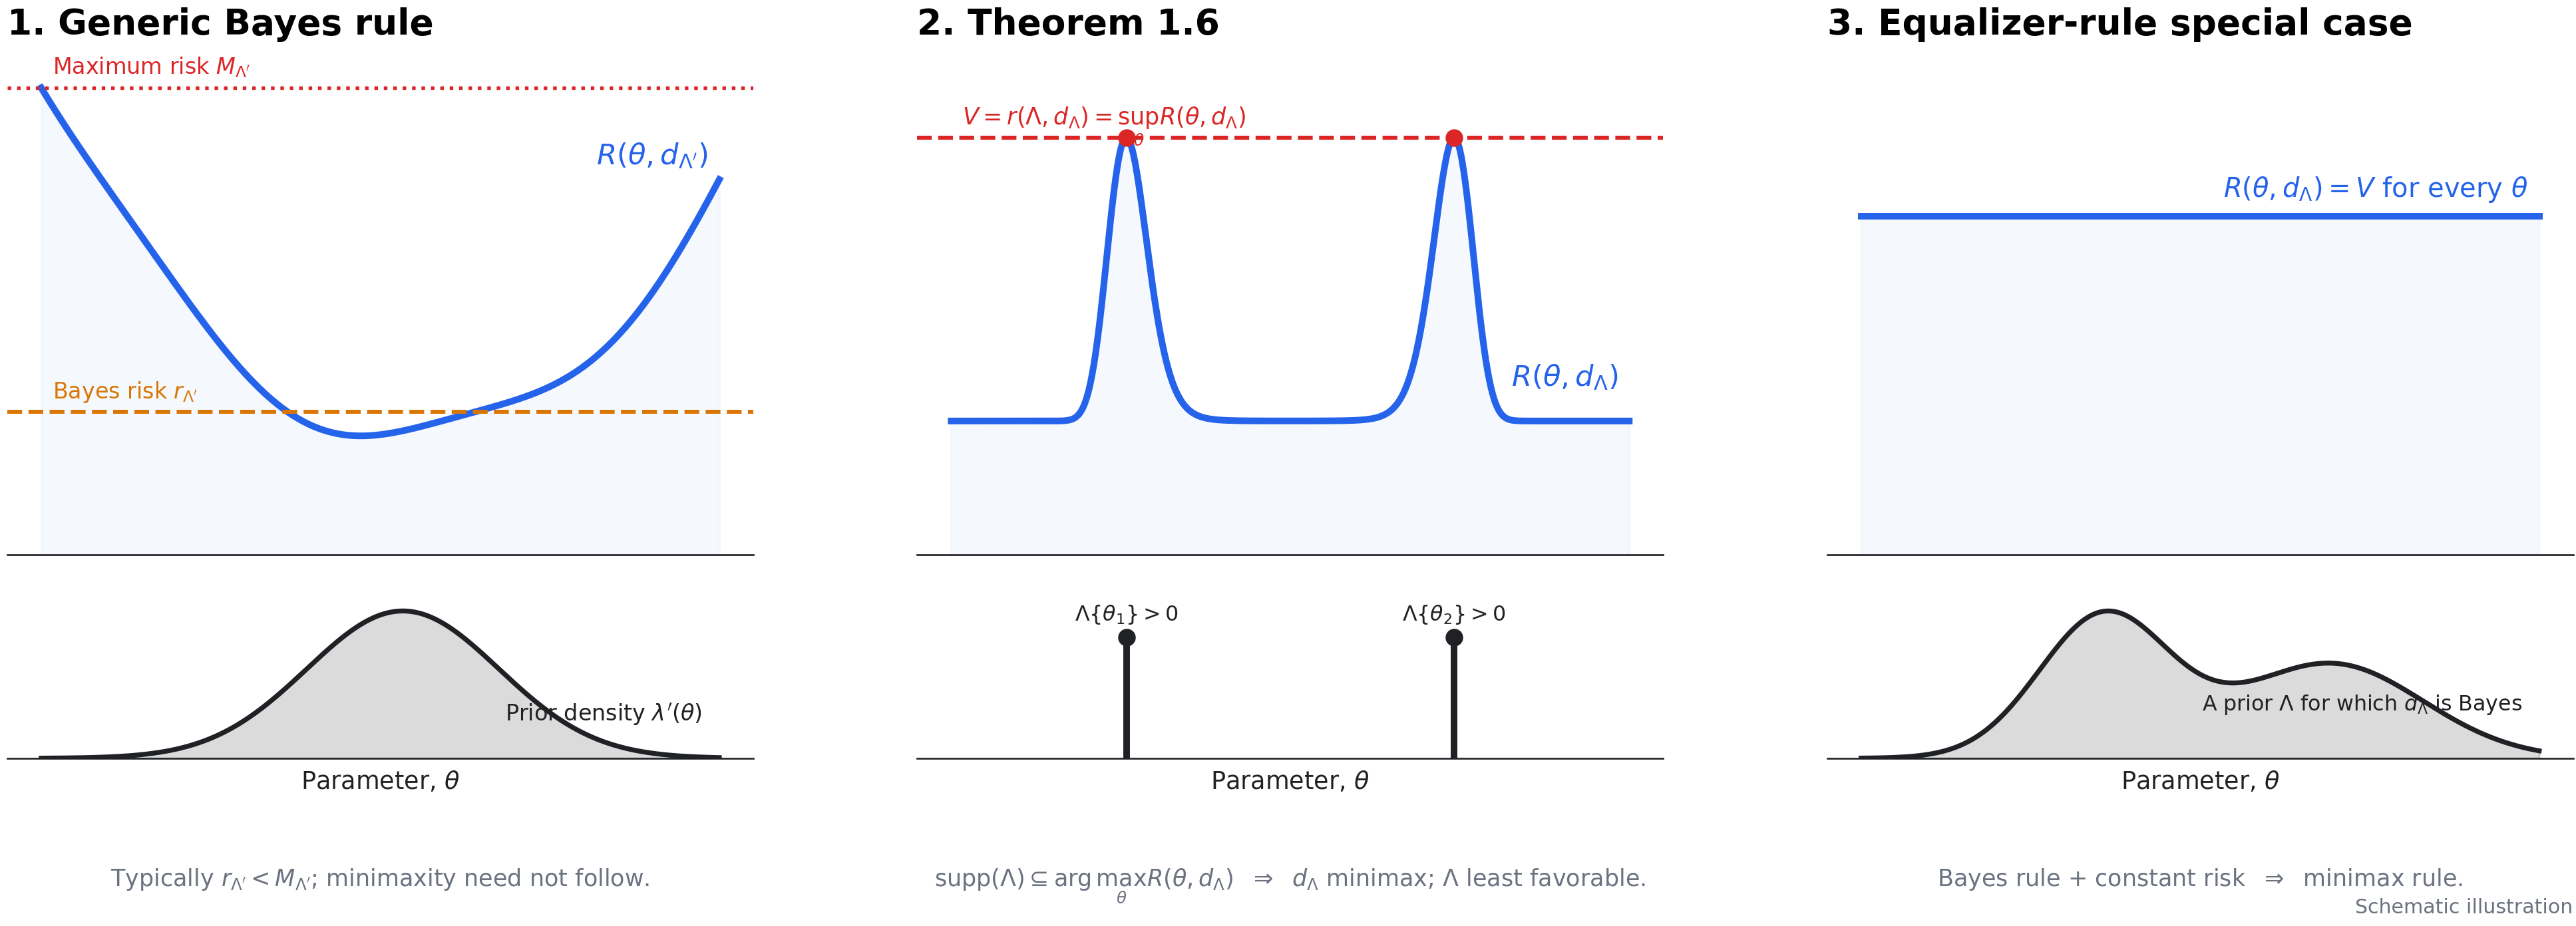
\includegraphics[width=0.9\linewidth]{figures/theorem-1.6.png}
    \caption{
    Intuition for Theorem 1.6. A generic Bayes rule need not be minimax (left). If the prior is concentrated on the maximum-risk points of its Bayes rule, that rule is minimax and the prior is least favorable (center). A constant-risk Bayes rule is a special equalizer case (right).
    }
    \label{fig:theorem-1.6}
\end{figure}


% --- other interpretations of Theorem 1.6, do not delete ---
% [Inaccurate. The theorem is a sufficient condition; it does not say that every minimax rule must arise this way.] In other words, \textbf{the minimax rule is the Bayes rule associated with the prior under which the Bayes risk is constant a.e in the parameter space} (equivalently, equals its maximum in the parameter space), and this prior is least favorable.\footnote{Not any constant risk can be minimax. It is minimax if it corresponds to a Bayes rule.}

% This is a delicate equilibrium: $\Lambda$ determines $d_\Lambda$, and the resulting risk $R(\theta, d_\Lambda)$ must attain its maximum where $\Lambda$ places its mass.





\begin{mybox}
    \textbf{Finding minimax rules.}
    \begin{enumerate}
        \item Direct method: find $d_M$ such that it attains the smallest worst-case risk, namely,
        \[
        \sup_{\theta \in \Theta} R(\theta, d_M) = \inf_{d \in \mathcal{D}} \sup_{\theta \in \Theta} R(\theta, d).
        \]
        Specifically, first find an expression for $\sup_\theta R(\theta, d)$ (parametrized by $d$), then find the $d$ that minimizes this maximum risk.
        \item Use Theorem 1.6 to find a Bayes rule $d_\Lambda$ such that $R(\Lambda, d_\Lambda) = \sup_{\theta \in \Theta} R(\theta, d_\Lambda).$
        \item \textbf{(Most useful)} If $d_\Lambda$ is Bayes with constant risk\footnote{A rule with constant risk is called an \emph{equalizer rule}.}, then $d_\Lambda$ is minimax.
        \begin{enumerate}[leftmargin=48pt]
            \item[Step 1:] Find the Bayes rule $d_\Lambda$ for a given class of prior distribution $\Lambda$'s.
            \item[Step 2:] Calculate the risk function $R(\theta, d_\Lambda)$ of $d_\Lambda$.
            \item[Step 3:] Find the cases (structure of the prior $\Lambda$) where $R(\theta, d_\Lambda)$ is independent of $\theta$, that is, where $R(\theta, d_\Lambda)$ is constant a.e. w.r.t. $\Lambda$.
            \item[Step 4:] These cases give the least favorable prior(s) $\Lambda$ and the minimax rule(s) $d_\Lambda$.
            \item[Remark:] \underline{The key is to show a rule is both a Bayes rule and an equalizer rule.} Alternatively, we can first find an equalizer rule $d^*$ such that $R(\theta, d^*)$ is constant in $\theta$, then show $d^*$ is Bayes with respect to some proper prior $\Lambda$. See Examples 1.21 \& 1.27.
        \end{enumerate}
        \item (Theorem 1.13, long-version notes) Construct a sequence of priors whose Bayes risks increase to a limit $r$; this lower-bounds the minimax risk by $r$. If you can find an estimator whose worst-case risk attains $r$, then it must be minimax, and the priors form a least favorable sequence. See Example 1.22.
        \item (Lemma 1.3, long-version notes) Prove that an estimator is minimax over a simpler subclass $P_0$, then extend the result to a larger class $P_1$ by showing that its worst-case risk remains unchanged when the model class is enlarged.
        The subclass $P_0$ is usually chosen to make the minimax risk finite.
        See Examples 1.23 \& 1.24.
    \end{enumerate}
\end{mybox}


% Bayes estimators with proper priors are minimax and admissible
% admissibility: pointwise dominance
% minimaxity: global dominance

\subsubsection{What types of decision rules are admissible?}
\begin{mybox}
\textbf{Finding admissible rules.}
\begin{enumerate}
    \item (By def.) Any decision rule $d$ that \emph{uniquely} minimizes $R(\theta, d)$ for \emph{some} $\theta \in \Theta$.
    \item (Minimax rules.) A \emph{unique} minimax rule is admissible.
    \item (Theorem 1.7: Bayes rules.) Any \emph{unique} Bayes rule with \emph{finite} Bayes risk is admissible. In other words, so long as a rule is \emph{uniquely} Bayes under \emph{some} prior distribution, it is admissible. 
    \footnote{Again, admissibility has nothing to do with the prior. It is admissible relative to the entire parameter space $\Theta$.}
    \\(Theorem 1.10: Bayes rules.) Any Bayes rule with \emph{finite} Bayes risk is admissible (uniqueness is no longer needed), given the conditions: (1) the risk function $R(\theta,d)$ is continuous in $\theta$ for all $d\in \mathcal{D}$, and (2) the prior $\Lambda$ gives positive probability to any open subset of $\Theta$. 
    \footnote{i.e., the support of $\Lambda$ is $\Theta$. This does not mean $\Lambda({\theta})>0$ for every $\theta$; a continuous prior distribution assigns zero probability to individual points while still having full support. Together with continuity, the positive-probability condition prevents a strict risk improvement on a set of $\Lambda$-measure zero, which yields the same Bayes risk but kills admissibility.}
    \footnote{The result also holds for generalized Bayes rule.}
    \item (Theorem 1.8: linear estimators.) Let $X$ have mean $\theta$ and variance $\sigma^2$. Under squared-error loss, a linear estimator $aX+b$ of $\theta$ is inadmissible if $a<0$, $a>1$, or $a=1$ with $b\neq 0$. Thus, the only potentially admissible linear estimators of $\theta$ are $\{X,\ b,\ aX+b\text{ with }0<a<1\}$, where every constant estimator $b$ is admissible and $X$ is admissible within the class of linear estimators.
    \footnote{For a random sample $X_1,\ldots,X_n$, the theorem applies to linear estimators $a\bar X+b$ by taking $X=\bar X$, for which $\E[\bar{X}] = \theta,\ \Var(\bar{X})=\sigma^2/n$.}
    \\(Theorem 1.9: sample mean estimator.) If $X_1, \ldots, X_n \stackrel{i.i.d.}{\sim} N(\theta, \sigma^2)$ with $\sigma^2$ known, then, under squared error loss, $\bar{X}$ is an admissible estimator of $\theta$.
    \footnote{More generally, let $X_1,\ldots,X_n \stackrel{i.i.d}{\sim} N_k(\mu,\Sigma)$, where $\Sigma$ is known and positive definite. Under squared-error loss, the sample mean $\bar{X}$ is admissible when $k\leq 2$ but inadmissible when $k\geq 3$; the latter result is the Stein phenomenon.}
\end{enumerate}
\end{mybox}


% trick: Theorem 1.9: continuity of risk fun. + contradiction b/w admissibility and bayes

\section{Miscellanea}

A more comprehensive collection of commonly used mathematical tools is available in the BIOS762 review notes.


\subsection{Common Bayesian results}
\begin{table}[!ht]
    \centering
    \begin{tabular}{l|l}
        \toprule
        \textbf{Loss function} & \textbf{Bayes rule} \\
        \midrule
        Weighted squared error loss: $L(\theta, a) = k(\theta) \|\theta-a\|_2^2$\quad & $d_\Lambda(x) = \frac{\E[k(\theta) \theta|X=x]}{\E[k(\theta)|X=x]}$ = posterior weighted mean\\
        \midrule
        Squared error loss: $L(\theta, a) = \|\theta-a\|_2^2$ &  $d_\Lambda(x) = \E[\theta | X=x]$ = posterior mean\\
        \midrule
        Absolute error loss: $L(\theta, a) = |\theta - a|$ & $d_\Lambda(x) = \text{median}(\theta|X=x)$ = posterior median\\
        \midrule
        0-1 loss: $L(\theta, a) = \mathbf{1}\{\theta \neq a\}$ & $d_\Lambda(x) = \argmax_\theta\ p(\theta|X=x)$ = posterior mode\\
        \bottomrule
    \end{tabular}
    \caption{Common Bayes rules.}
    \label{tab:common_bayes_rules}
\end{table}

\textbf{Notes:}
\begin{itemize}
    \item If $L(\theta,a)$ is convex in $a$ (for every fixed $\theta$), it suffices to consider only deterministic Bayes rules.
    \item If $L(\theta,a)$ is strictly convex in $a$ and posterior expected loss $\E_{\theta|X}[L(\theta,a)|X=x]$ is finite for some $a$, then the Bayes estimator is unique.
\end{itemize}



\begin{sidewaystable}[p]
\centering
\small
\renewcommand{\arraystretch}{1.15}
\setlength{\tabcolsep}{4pt}

\begin{tabular}{%
>{\raggedright\arraybackslash}p{0.10\linewidth}
>{\raggedright\arraybackslash}p{0.16\linewidth}
>{\raggedright\arraybackslash}p{0.06\linewidth}
>{\raggedright\arraybackslash}p{0.18\linewidth}
>{\raggedright\arraybackslash}p{0.40\linewidth}}
\toprule
\textbf{Conjugate pair} &
\textbf{Sampling model} &
\textbf{Unknown} &
\textbf{Prior (loss)} &
\textbf{Posterior / mean / Bayes rule / Bayes risk} \\
\midrule

\textbf{Normal--Normal} (mean, $\sigma^2$ known)
&
$x_1,\dots,x_n\mid\theta \overset{iid}{\sim} N(\theta,\sigma^2)$
&
$\theta$
&
$\theta\sim N(\mu_0,\tau_0^2)$;\quad $L(\theta,a)=(\theta-a)^2$
&
\parbox[t]{\linewidth}{%
Posterior: $\theta\mid x\sim N(\mu_n,\tau_n^2)$,\;
$\tau_n^2=\big(\tfrac{1}{\tau_0^2}+\tfrac{n}{\sigma^2}\big)^{-1}$.\\
Mean: $\mu_n=w\mu_0+(1-w)\bar x$, \;
$w=\dfrac{1/\tau_0^2}{1/\tau_0^2+n/\sigma^2}=\dfrac{\sigma^2}{\sigma^2+n\tau_0^2}$.\\
Bayes rule: $d_B(x)=\mu_n$.\\
Bayes risk: $r_B=\E[\Var(\theta\mid X)]=\tau_n^2=\dfrac{\tau_0^2\sigma^2}{\sigma^2+n\tau_0^2}$.} \\

\midrule

\textbf{Binomial--Beta} (proportion)
&
$Y\mid p\sim \mathrm{Bin}(n,p)$
&
$p$
&
$p\sim \mathrm{Beta}(\alpha,\beta)$;\quad $L(p,a)=(p-a)^2$
&
\parbox[t]{\linewidth}{%
Posterior: $p\mid y\sim \mathrm{Beta}(\alpha+y,\beta+n-y)$.\\
Mean: $\E[p\mid y]=\dfrac{\alpha+y}{\alpha+\beta+n}
= w\,\dfrac{\alpha}{\alpha+\beta}+(1-w)\,\dfrac{y}{n}$,\;
$w=\dfrac{\alpha+\beta}{\alpha+\beta+n}$.\\
Bayes rule: $d_B(y)=\E[p\mid y]$.\\
Bayes risk: $r_B=\E[\Var(p\mid Y)]
=\dfrac{\alpha\beta}{(\alpha+\beta)(\alpha+\beta+1)(\alpha+\beta+n)}$.} \\

\midrule


\textbf{Poisson--Gamma} (rate)
&
$X_1,\dots,X_n\mid \lambda \overset{iid}{\sim} \mathrm{Pois}(\lambda)$
&
$\lambda$
&
$\lambda\sim \mathrm{Gamma}(a,b)$ (shape/rate);\quad $L(\lambda,a_0)=(\lambda-a_0)^2$
&
\parbox[t]{\linewidth}{%
Let $S=\sum_{i=1}^n x_i$. Posterior:
$\lambda\mid x\sim \mathrm{Gamma}(a+S,b+n)$.\\
Mean: $\E[\lambda\mid x]=\dfrac{a+S}{b+n}
= w\,\dfrac{a}{b}+(1-w)\,\bar x$,\;
$w=\dfrac{b}{b+n}$.\\
Bayes rule: $d_B(x)=\E[\lambda\mid x]$.\\
Bayes risk: $r_B=\E[\Var(\lambda\mid X)]
=\E\big[\tfrac{a+S}{(b+n)^2}\big]=\dfrac{a}{b(b+n)}$.} \\

\midrule

\textbf{Exponential--Gamma} (rate)
&
$X_i\mid \lambda \overset{iid}{\sim} \mathrm{Exp}(\lambda)$
&
$\lambda$
&
$\lambda\sim \mathrm{Gamma}(a,b)$;\quad $L(\lambda,a_0)=(\lambda-a_0)^2$
&
\parbox[t]{\linewidth}{%
Let $T=\sum_{i=1}^n x_i$. Posterior:
$\lambda\mid x\sim \mathrm{Gamma}(a+n,b+T)$.\\
Mean: $\E[\lambda\mid x]=\dfrac{a+n}{b+T}$.\\
Bayes rule: $d_B(x)=\E[\lambda\mid x]$.\\
Bayes risk: $r_B=\E[\Var(\lambda\mid X)]
=\E\big[\tfrac{a+n}{(b+T)^2}\big]$.} \\

\midrule

\textbf{Multinomial--Dirichlet}
&
$(Y_1,\dots,Y_K)\mid \mathbf p\sim \mathrm{Mult}(n,\mathbf p)$
&
$\mathbf p$
&
$\mathbf p\sim \mathrm{Dir}(\alpha_1,\dots,\alpha_K)$;\quad
$L(\mathbf p,\mathbf a)=\sum_{i=1}^K(p_i-a_i)^2$
&
\parbox[t]{\linewidth}{%
Let $\alpha_0=\sum_{i=1}^K\alpha_i$. Posterior:
$\mathbf p\mid \mathbf y\sim \mathrm{Dir}(\alpha_1+y_1,\dots,\alpha_K+y_K)$.\\
Mean: $\E[p_i\mid \mathbf y]=\dfrac{\alpha_i+y_i}{\alpha_0+n}
= w\,\dfrac{\alpha_i}{\alpha_0}+(1-w)\,\dfrac{y_i}{n}$,\;
$w=\dfrac{\alpha_0}{\alpha_0+n}$.\\
Bayes rule: $d_{B,i}(\mathbf y)=\E[p_i\mid \mathbf y]$.\\
Bayes risk: $r_B=\E\big[\sum_{i=1}^K\Var(p_i\mid \mathbf Y)\big]
=\dfrac{\alpha_0^2-\sum_{i=1}^K\alpha_i^2}{\alpha_0(\alpha_0+1)(\alpha_0+n)}$.} \\

\bottomrule
\end{tabular}
\caption{Common conjugate Bayes rules and Bayes risks under squared-error loss.}
\label{tab:conjugate-bayes}
\end{sidewaystable}




\end{document}
